\documentclass[12pt]{article}

\usepackage{amsmath}
\usepackage{amssymb}
\usepackage{graphicx}
\usepackage{pgfplots}

\graphicspath{/images}
\pgfplotsset{compat=1.18}

\title{Probability And Statistics}
\author{Thomas Vroom}

\begin{document}
\maketitle
\pagenumbering{gobble}

%
% Lecture 1
%
\section*{Lecture 1: Probability and Counting}
\textbf{Sample Space} $S$ of an experiment is the set of all possible outcomes of the experiment.
An \textbf{event} $A$ is a subset of sample space $S$, we say $A$ \textbf{occured} if the actual outcome of the experiment is in $A$.

\[ P(A) = \frac{|A|}{|S|} \]

\noindent
The probability of something happening is the events satisfying that outcome over the total number of outcomes.
Formulas that follow from this include $P(\varnothing) = 0$ and $P(S) = 1$.

\noindent
\\
\textbf{Sampling table}: choose $k$ objects out of $n$

\begin{table}[h]
    \centering
    \begin{tabular}{lll}
    & \textbf{order matters} & \textbf{order doesn't matter} \\
    \textbf{with replacement} & $n^k$ & $\binom{n+k-1}{k}$ \\
    \textbf{without replacement} & $\frac{n!}{k!}$ & $\binom{n}{k}$
    \end{tabular}
\end{table}

\noindent
Further formulas:

\[ P(A^c) = 1 - P(A) \]
\[ P(A \cap B) = P(A) \cdot P(B) \]
\[ P(A \cup B) = P(A) + P(B) \]

%
% Lecture 2
%
\section*{Lecture 2: Conditional Probability}
$P(A|B)$ is the \textbf{posterior probability} of $A$.
Assuming $P(B) > 0$, $P(A|B)$ is the probability of $A$ given the evidence $B$.
\textbf{$A|B$ is not an event!!!}

\[ P(A|B) = \frac{P(A \cap B)}{P(B)} = \frac{P(B|A)P(A)}{P(B)} \]

\noindent
\textbf{The Law of Total Probability:}

\[ P(B) = \sum_{i = 1}^{n} P(B|A_i)P(A_i) \]

\begin{figure}[h]
    \centering
    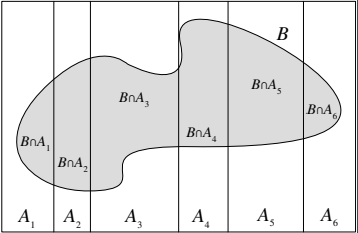
\includegraphics{images/lawoftotalprobability.PNG}
\end{figure}

%
% Lecture 3
%
\section*{Lecture 3: Random Variables}
A \textbf{Random Variable} maps the sample space onto the real number line.
The \textbf{Probability Mass Function (PMF)} is a function that describes the distribution of a random variable $X$.
This is formally given by:

\[ P(X = x) = \{s \in S : X(s) = x\} \]

\noindent
Here $X$ is the random variable, $S$ is the sample space, and $x$ is a real number.

\newpage
\noindent
\\
\textit{Example:}
Consider an experiment where we toss a coin twice.
The sample space is $S = \{HH, HT, TH, TT\}$.
Let random variable $X$ be the number of heads.
This defines random variable $X$ as:

\[ X(TT) = 0, X(TH) = X(HT) = 1, X(HH) = 2 \]

\noindent
The PMF is defined as:

\[ P(X = 0) = \frac{1}{4}, P(X = 1) = \frac{1}{2}, P(X = 2) = \frac{1}{4} \]

\pgfplotstableread[row sep=\\,col sep=&]{
    interval & p \\
    -1 & 0 \\
    0 & 0.25 \\
    1 & 0.5 \\
    2 & 0.25 \\
    3 & 0 \\
}\PMFCoinToss

\begin{center}
    \begin{tikzpicture}
        \begin{axis}[
                ybar,
                symbolic x coords={-1,0,1,2,3},
                xtick=data,
                ymin=0,ymax=1,
                ylabel={$P(X=x)$},
                xlabel={$X=x$}
            ]
            \addplot table[x=interval,y=p]{\PMFCoinToss};
        \end{axis}
    \end{tikzpicture}
\end{center}

\noindent
\\
Random variable: maps from sample space $S$ to real number $\mathbb{R}$\\
PMF: maps real number $\mathbb{R}$ to probability $[0,1]$

\noindent
\\
A PMF is \textit{valid} if:

\begin{itemize}
    \item it is nonnegative (no negative probabilities)
    \item it sums to 1
\end{itemize}

\newpage
\noindent
\underline{\textbf{Named Distributions:}}

\[ X \sim \text{Bern}(p) \]

\noindent
\textbf{Bernoulli Distribution:} $X$ has a Bernoulli distribution if there are only two outcomes possible, with the probability for success being $p$.
This means $P(X = 1) = p$ and $P(X = 0) = 1 - p$.

\begin{center}
    $-----------------------------------------$
\end{center}

\[ X \sim \text{Bin}(n, p) \]

\noindent
\textbf{Binomial Distribution:} $X$ has a binomial distribution if $n$ independent Bernoulli trails with success probability $p$ are performed.
Here $X$ represents the number of successes.
The PMF for a binomial distribution equals:

\[ P(X = k) = \binom{n}{k} p^k (1 - p)^{n - k} \]

\begin{center}
    $-----------------------------------------$
\end{center}

\[ X \sim \text{DUnif}(C) \]

\noindent
\textbf{Discrete Uniform Distribution:} $X$ has a discrete uniform distribution if $X$ has equal possibility to be any real number defined in set $C$.
The PMF for a discrete uniform distribution equals $P(X = x) = \frac{1}{|C|}$ for $x \in C$ (else 0).

\newpage
\noindent
The \textbf{Cumulative Distribution Function (CDF)} of a random variable $X$ is given by the function $F_X(x) = P(X \leq x)$.  

\begin{figure}[h]
    \centering
    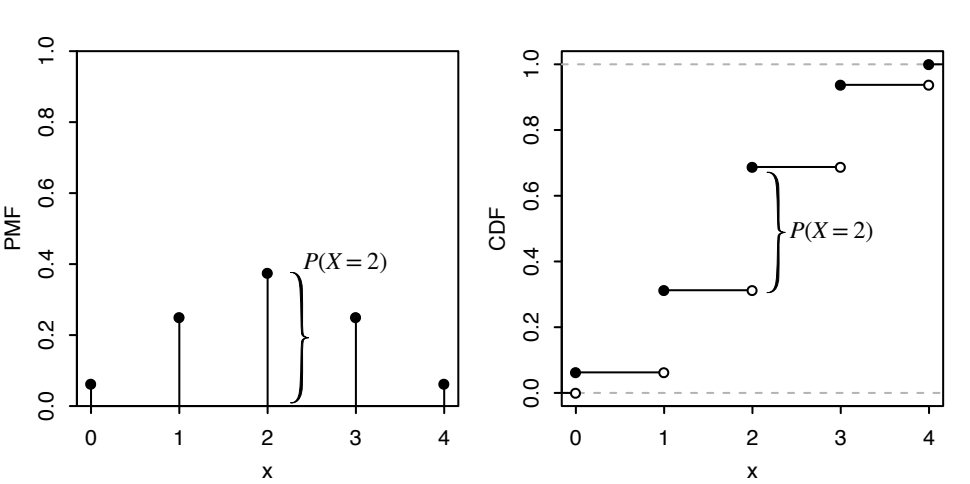
\includegraphics[scale=0.6]{images/pmfcdf.PNG}
\end{figure}

\noindent
Any CDF has the following properties:

\begin{itemize}
    \item It is increasing
    \item It is right-continuous
    \item $\lim_{x \to -\infty} F_X(x) = 0$
    \item $\lim_{x \to \infty} F_X(x) = 1$
\end{itemize}

\begin{figure}[h]
    \centering
    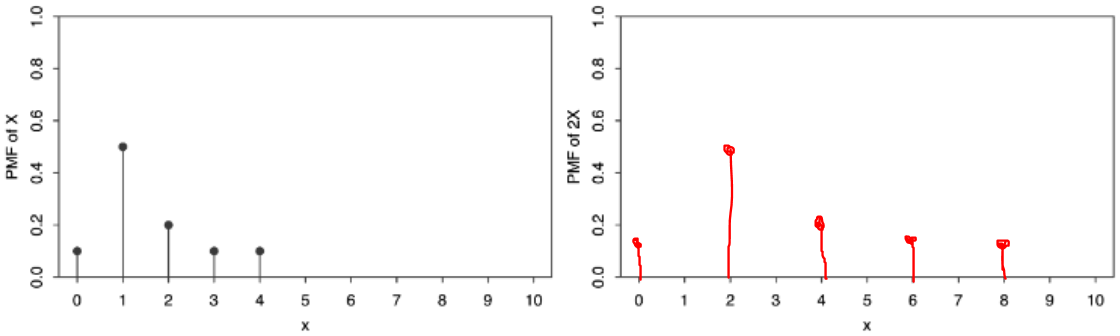
\includegraphics[scale=0.55]{images/rvfunction.PNG}
    \caption{Multiplication of Random Variables}
    \label{fig:1}
\end{figure}

%
% Lecture 4
%
\section*{Lecture 4: Expectation}
The \textbf{Expected Value} (also called expectation or mean) of a random variable $X$ is defined as:

\[ E(X) = \sum_{i = 1}^{\infty} x_i P(X = x_i) \]

\noindent
Here $P(X = x_i)$ is refered to as the \textbf{weight} of that value of $x$.
If random variables $X$ and $Y$ have the same distribution then they also have the same expectation, but two variables don't \textit{need} to have the same distribution to have the same expectation:

\begin{figure}[h]
    \centering
    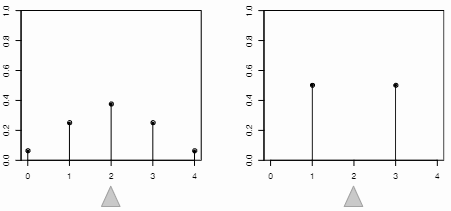
\includegraphics{images/sameexpectation.PNG}
\end{figure}

\noindent
For any two random variables $X$ and $Y$, and any constant $c$:

\[ E(X) + E(Y) = E(X + Y) \]

\[ E(cX) = c \cdot E(X) \]

\noindent
\textbf{Law of the Unconscious Statestician:}

\[ E(g(X)) = \sum_{x}^{} g(x)P(X = x) \]

\newpage
\noindent
\textit{Example:}
Let random variable $X$ be defined for $0, 1, 2, ...$ with probabilities $p_0, p_1, p_2, ...$ so its PDF equals $P(X = n) = p_n$.
Then $X^3$ is defined for $0^3, 1^3, 2^3, ...$ with probabilities $p_0, p_1, p_2, ...$ (see figure \ref{fig:1}).
This gives:

\[ E(X) = \sum_{n = 0}^{\infty} n \cdot p_n \]

\[ E(X^3) = \sum_{n = 0}^{\infty} n^3 \cdot p_n \]

\noindent
\textbf{Variance:}

\[ \text{Var}(X) = E(X^2) - E(X)^2 \]

\noindent
\textbf{Standard Deviation:}

\[ \text{SD}(X) = \sqrt{\text{Var}(X)} \]

\noindent
\textbf{Poisson Distribution:}

\[ X \sim \text{Pois}(\lambda) \]

\noindent
$X$ has a Poisson distribution defined by a parameter $\lambda$.
If $X$ has a Poisson distribution then $E(X) = \lambda$ and Var$(X) = \lambda$.
Its PMF is:

\[ P(X = k) = \frac{e^{-\lambda}\lambda^k}{k!} \]

\noindent
Let $A_1, ... , A_n$ be events with $P(A_i) = p_i$.
You can use a Poisson distribution if $n$ is large and $p_i$ is small.
The $\lambda$ for this distribution is the average number of occurences (expected value) $\lambda = n \cdot p_i$.

%
% Lecture 5
%
\newpage
\section*{Lecture 5: Continuous Random Variables}
A random variable has a continuous distribution if its CDF is differentiable.
The CDF can be undifferentiable at various (end)points, as long as it is differentiable everywhere else.
The PMF of a continuous random variable is called a \textbf{probability density function (PDF)}.

\begin{figure}[h]
    \centering
    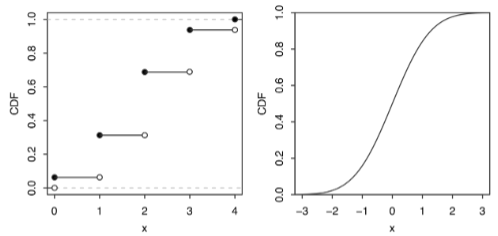
\includegraphics{images/continuouscdf.PNG}
    \caption{CDF with discrete r. v. (left) and continuous r. v. (right)}
\end{figure}

\noindent
For a continuous random variable $X$, the \textit{PDF} of $X$ is the derivative of the \textit{CDF} of $X$.
Vice versa, the \textit{CDF} of $X$ is the integral of the \textit{PDF} of $X$.

\begin{figure}[h]
    \centering
    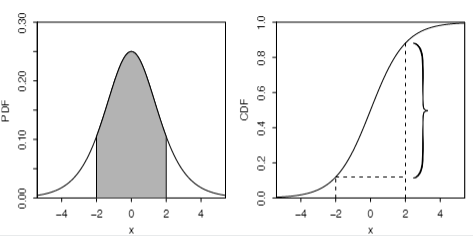
\includegraphics{images/pmfintegral.PNG}
\end{figure}

\noindent
For a continuous random variable $X$, $P(a < X < b)$ equals the area under the graph of the PDF of $X$.
Thus, $P(a < X < b) = \int_{a}^{b} f_X(x) \,dx$ where $f_X(x)$ is the PDF of $X$.

\newpage
\noindent
To calculate the \textbf{expected value} of a continuous random variable, use the same formulas as a discrete random variable, but use an integral ($\int_{-\infty}^{\infty}$) instead of a sum.
For a PDF of a continuous random variable to be valid, it must be:

\begin{itemize}
    \item nonnegative
    \item integrate to 1 ($\int_{-\infty}^{\infty} f(x) \,dx = 1$)
\end{itemize}

\noindent
\textbf{Uniform Distribution:}

\[ X \sim \text{Unif}(a, b) \]

\noindent
$X$ has a uniform distribution if its PDF is $\frac{1}{b-a}$ if $a < x < b$, else 0.

\begin{figure}[h]
    \centering
    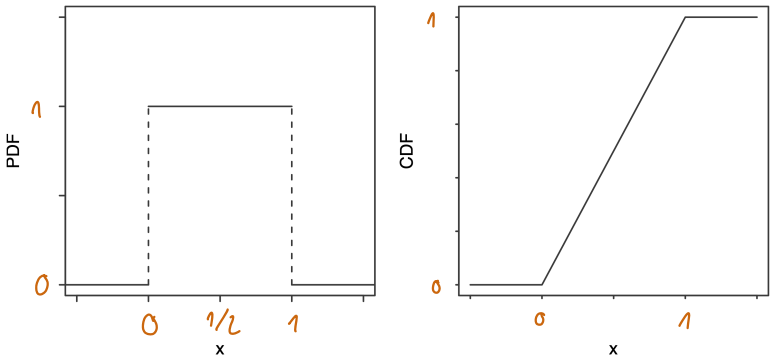
\includegraphics[scale=0.7]{images/uniformdistribution.PNG}
    \caption{$X \sim \text{Unif}(0, 1)$}
\end{figure}

\noindent
\textbf{Standard Normal Distribution:}

\[ Z \sim N(0, 1) \]

\noindent
A continuous random variable $Z$ is said to have the standard normal distribution if its PDF ($\varphi$) is given by:

\[ \varphi(z) = \frac{1}{\sqrt{2\pi}} e^{-z^2/2} \]

\noindent
for $-\infty < z < \infty$.

\newpage
\noindent
The standard normal CDF ($\phi$) is the area under the standard normal PDF ($\varphi$):

\[ \phi(z) = \int_{-\infty}^{z} \varphi(t) \,dt = \int_{-\infty}^{z} \frac{1}{\sqrt{2\pi}} e^{-t^2/2} \,dt  \]

\begin{figure}[h]
    \centering
    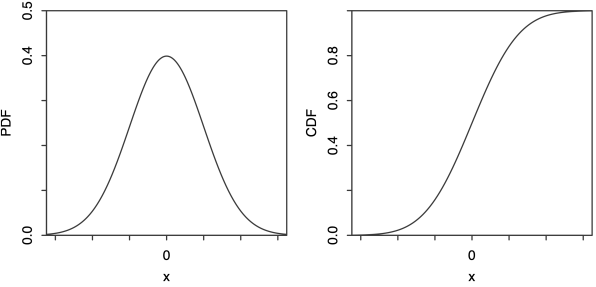
\includegraphics{images/normaldistribution.PNG}
\end{figure}

\noindent
Notice the symmetry of the PDF around 0.
This means $Z$ has an expected value of $E(Z) = 0$ and a variance of $\text{Var}(Z) = 1$.

\noindent
\\
If $Z \sim N(0, 1)$, then $X = \mu + \sigma Z$ is said to have a normal distribution with mean $\mu$, variance $\sigma^2$ and standard deviation $\sigma$, for any real $\mu$ and $\sigma > 0$.
This is denoted as:

\[ X \sim N(\mu, \sigma^2) \]

%
% Lecture 6
%
\newpage
\section*{Lecture 6: Joint Distributions}
The \textbf{joint PMF} of discrete random variables $X$ and $Y$ is defined as \\$P(X = x, Y = y)$.
The \textbf{marginal PMF} of discrete random variables $X$ and $Y$ equals:

\[ P(X = x) = \sum_{y} P(X = x, Y = y) \]

\noindent
The \textbf{conditional PMF} of discrete random variable $Y$ given $X = x$ is:

\[ P(Y = y | X = x) = \frac{P(X = x, Y = y)}{P(X = x)} \]

\noindent
If random variables $X$ and $Y$ are \textbf{independent} and \textbf{discrete}, then:

\[ P(X = x, Y = y) = P(X = x) \cdot P(Y = y) \]

\noindent
\textit{Example:}
Suppose we have researched a small portion of the population on the effects of smoking.
Random variables $X$ and $Y$ are both Bernoulli distributed.
$X = 0$ represents a non-smoker, $X = 1$ represents a smoker.
$Y = 0$ means they are not developing cancer, $Y = 1$ means they are developing cancer.
For this research $n = 100$.

\begin{table}[h]
    \centering
    \begin{tabular}{lll}
    & Y = 0 (no cancer) & Y = 1 (cancer) \\
    X = 0 (non smoker) & 72 & 3 \\
    X = 1 (smoker) & 20  & 5
    \end{tabular}
\end{table}

\noindent
Some examples:

\begin{itemize}
    \item $P(X = 0, Y = 0) = \frac{72}{100}$ (non smoker has no cancer)
    \item $P(X = 1, Y = 1) = \frac{5}{100}$ (smoker has cancer)
    \item $P(X = 1) = \frac{20}{100} + \frac{5}{100} = \frac{25}{100}$ (number of smokers)
    \item $P(Y = 1 | X = 1) = \frac{P(X = 1, Y = 1)}{P(X = 1)} = \frac{5/100}{25/100} = \frac{1}{5}$ (cancer if smoker)
    \item $P(Y = 1 | X = 0) = \frac{P(X = 0, Y = 1)}{P(X = 0)} = \frac{3/100}{75/100} = \frac{1}{25}$ (cancer if non smoker)
    \item $P(X = 1, Y = 1) \neq P(X = 1) \cdot P(Y = 1)$, thus $X$ and $Y$ are \textit{not} independent of each other.
\end{itemize}

\newpage
\noindent
For continuous joint PDF $f_{X, Y}$:

\[ \int_{-\infty}^{\infty} \int_{-\infty}^{\infty} f_{X, Y}(x, y) \,dx \,dy = 1 \]

\noindent
If $X$ and $Y$ are continuous with joint CDF $F_{X, Y}$, then their joint PDF is the derivative of the joint CDF $F_{X, Y}$ with respect to x and y.
For joint PDF $f_{X, Y}$, the marginal PDF equals:

\[ P(X = x) = \int_{-\infty}^{\infty} f_{X, Y}(x, y) \,dy \]

\noindent
The conditional PDF is calculated the same as the conditional PMF.

\noindent
\\
\textbf{2D LOTUS:}
Let $g$ be a function from $\mathbb{R}^2$ to $\mathbb{R}$.
If random variables $X$ and $Y$ are discrete:

\[ E(g(X, Y)) = \sum_x \sum_y g(x, y) P(X = x, Y = y) \]

\noindent
If $X$ and $Y$ are continuous with joint PDF $f_{X, Y}$:

\[ E(g(X, Y)) = \int_{-\infty}^{\infty} \int_{-\infty}^{\infty} g(x, y) f_{X, Y}(x, y) \,dx \,dy \]

\noindent
The \textbf{covariance} between random variables $X$ and $Y$ is defined as:

\[ \text{Cov}(X, Y) = E(XY) - E(X)E(Y) \]

\noindent
This also means $\text{Cov}(X, X) = \text{Var}(X)$.
If $\text{Cov}(X, Y) = 0$, then $X$ and $Y$ are \textbf{independent}.
The \textbf{correlation} between $X$ and $Y$ is:

\[ \text{Corr}(X, Y) = \frac{\text{Cov}(X, Y)}{\sqrt{\text{Var}(X)\text{Var}(Y)}} \]

\[ \text{Corr}(X, Y) \in [-1, 1] \]

\noindent
A $k$-dimensional vector $X = (X_1, ... , X_k)$ has a \textbf{multivariate normal distribution} if every linear combination of $X$ has a normal distribution.
This means $t_1 X_1, ... , t_k X_k$ has a normal distribution for any constants $t_1, ... , t_k$.

%
% Lecture 7
%
\newpage
\section*{Lecture 7: Moments}
The \textbf{Median} of a random variable $X$ is the exact midpoint of its probability.

\[ P(X \leq c) \geq \frac{1}{2} \text{  and  } P(X \geq c) \geq \frac{1}{2} \]

\noindent
Half of the distribution falls to the left of $c$, the other half to the right of $c$.
The means the CDF of $X$ hits $\frac{1}{2}$ exactly at $c$ (assuming it has no jumps).

\pgfplotstableread[row sep=\\,col sep=&]{
    interval & p \\
    1 & 0.2 \\
    2 & 0.2 \\
    3 & 0.2 \\
    4 & 0.2 \\
    5 & 0 \\
    6 & 0 \\
    7 & 0 \\
    8 & 0 \\
    9 & 0 \\
    10 & 0.2 \\
}\PMFExpectedMean

\begin{figure}[h]
    \centering
    \begin{tikzpicture}
        \begin{axis}[
                ybar,
                symbolic x coords={1,2,3,4,5,6,7,8,9,10},
                xtick=data,
                ymin=0,ymax=1,
                ylabel={$P(X=x)$},
                xlabel={$X=x$}
            ]
            \addplot table[x=interval,y=p]{\PMFExpectedMean};
        \end{axis}
    \end{tikzpicture}
    \caption{$E(X) = 4$, Median$(X) = 3$}
\end{figure}


\noindent
\textbf{Moments:}
Let $X$ be a random variable with mean $\mu$ and variance $\sigma^2$:

\begin{itemize}
    \item the $n$th \textbf{moment} of $X$ is $E(X^n)$
    \item the $n$th \textbf{central moment} of $X$ is $E((X - \mu)^n)$
    \item the $n$th \textbf{standardized moment} of $X$ is $E((\frac{X - \mu}{\sigma})^n)$
\end{itemize}

\noindent
These moments can also not exist.
The \textbf{Moment Generating Function (MGF)} of a random variable is:

\[ M(t) = E(e^{tX}) \]

\noindent
This MGF exists if $M(t)$ is finite on some open interval $(-a, a)$ containing 0.
We can calculate the $n$th moment of $X$ by evaluating the $n$th derivative of the MGF at 0:

\[ E(X^n) = M^{(n)}(0) \]

\noindent
If two random variables $X$ and $Y$ have the same MGF, they must have the same distribution.
If $X$ and $Y$ are independent, then the MGF of $X + Y$ is the product of the individual MGFs:

\[ M_{X + Y}(t) = M_X(t) M_Y(t) \]

%
% Lecture 8
%
\section*{Lecture 8: Inequalities and Limits}
\textbf{Markov's inequality} states that for any random variable $X$ and a constant $a > 0$:

\[ P(|X| \geq a) \leq \frac{E|X|}{a} \]

\noindent
\textit{Example:} In a group of 100 people, is it possible that more than 50\% are richer than at least twice the average (mean) person?
This can be expressed as:

\[ P(|X| \geq 2E(X)) \leq \frac{1}{2} \]

\noindent
\textbf{Chebyshev's inequality} states that for any random variable $X$ with mean $\mu$ and variance $\sigma^2$, and a constant $a > 0$:

\[ P(|X - \mu| \geq a) \leq \frac{\sigma^2}{a^2} \]

\noindent
For all positive integers $n$, let

\[ \bar{X}_n = \frac{X_1 + ... + X_n}{n} \]

\noindent
The \textbf{Weak Law of Large Numbers} states that for all $\epsilon > 0$:

\[ P(|\bar{X}_n - \mu| \geq \epsilon) \to 0 \text{ as } n \to \infty \]

\newpage
\noindent
\textbf{Central Limit Theorem:}

\[ \text{As } n \to \infty \text{, } \sqrt{n} \left( \frac{\bar{X}_n - \mu}{\sigma} \right) \to N(0, 1) \text{ in distribution} \]

\noindent
For large $n$, the distribution of $\bar{X}_n$ is approximately $N(\mu, \frac{\sigma^2}{n})$.

\begin{figure}[h]
    \centering
    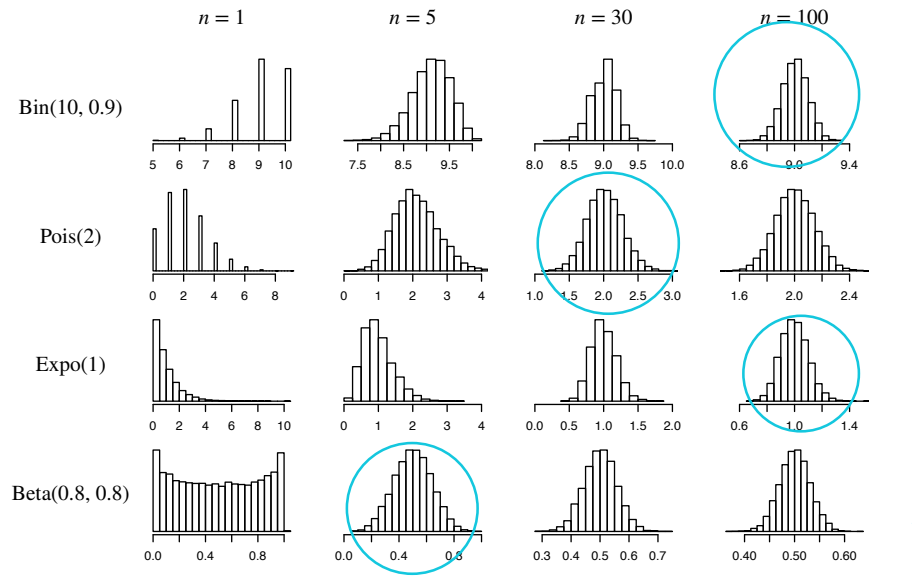
\includegraphics[scale=0.7]{images/sampledistributions.PNG}
\end{figure}

%
% Lecture 9
%
\newpage
\section*{Lecture 9: Population and Samples}
\textbf{Population Mean:}

\[ \mu = \frac{1}{N} \sum_{i = 1}^{N} x_i \]

\noindent
\textbf{Population Total:}

\[ \tau = \sum_{i = 1}^{N} x_i = N \mu \]

\noindent
\textbf{Population Variance:}

\[ \sigma^2 = \frac{1}{N} \sum_{i = 1}^{N} (x_i - \mu)^2 \]

\noindent
\textbf{Sample surveys} are used to obtain information about a large population by examining only a small fraction of that population.
A \textbf{sample} is a subset of population $N$ picked without replacement.
We can estimate the population mean $\mu$ by calculating the \textbf{sampling mean} $\bar{X}_n$:

\[ \bar{X}_n = \frac{1}{n} \sum_{i = 1}^{n} x_i \]

\noindent
The \textbf{sampling distribution} of $\bar{X}_n$ determines how accurately $\bar{X}_n$ estimates $\mu$.
For simple random sampling:

\[ E(\bar{X}) = \mu \]

\noindent
In general, if an estimator $\hat{\theta}$ of a population parameter $\theta$ is $E(\hat{\theta}) = \theta$, then $\hat{\theta}$ is \textbf{unbiased}.

\newpage
\noindent
In case of sampling \textit{with} replacement (total independence):

\[ \text{Var}(\bar{X}_n) = \frac{\sigma^2}{n} \]

\noindent
With \textbf{standard error}:

\[ \sigma_{\bar{X}_n} = \frac{\sigma}{\sqrt{n}} \]

\noindent
In case of sampling \textit{without} replacement (some dependences):

\[ \text{Var}(\bar{X}_n) = \frac{\sigma^2}{n} \left( 1 - \frac{n - 1}{N - 1} \right) \approx \frac{\sigma^2}{n} \]

\noindent
With \textbf{standard error}:

\[ \sigma_{\bar{X}_n} = \frac{\sigma}{\sqrt{n}} \sqrt{1 - \frac{n - 1}{N - 1}} \]

\noindent
If $n$ is large, but still small relative to $N$, then $\bar{X}_n$ is approximately normal distributed.

\noindent
\\
\textbf{Confidence Interval:}
For what upper bounds $u$ and $v$ is the probability of random variable $X$ a certain $1 - \alpha$:

\[ P(u \leq X \leq v) = 1 - \alpha \]

\[ u, v = \bar{X}_n \pm z(\alpha / 2) \cdot \sigma_{\bar{X}_n} \]

\noindent
For the following $z$-values:

\begin{table}[h]
    \centering
    \begin{tabular}{ll}
    $\alpha$ & $z$ \\
    0.10 & 1.65 \\
    0.05 & 1.96 \\
    0.01 & 2.58
    \end{tabular}
\end{table}

%
% Lecture 10
%
\newpage
\section*{Lecture 10: Parameter Estimation}
\textbf{Sample Moment:}

\[ \hat{\mu}_k = \frac{1}{n} \sum_{i = 1}^{n} X^k_i \]

\noindent
$\hat{\mu}_k$ is an estimate of the actual $k$th moment $\mu_k = E(X^k)$.

\noindent
\\
The \textbf{likelihood} of parameter $\theta$ is the probability of given data $x_1, x_2, ... , x_n$, that $\theta$ is a parameter of this data:

\[ \text{lik}(\theta) = f(x_1, x_2, ... , x_n | \theta) \]

\noindent
If the $X_i$ are independent and identically distributed, then:

\[ \text{lik}(\theta) = \prod_{i = 1}^{n} f(x_i | \theta) \]

\noindent
The \textbf{Maximum Likelihood Estimate} equals the maximum of:

\[ \sum_{i = 1}^{n} \log \left[ f(x_i | \theta) \right] \]

\noindent
\textbf{Consistent estimate}: $\hat{\theta}$ converges to $\theta$ as $n \rightarrow \infty$.

\noindent
\\
\textit{Example of MLE:}

\noindent
Let $X_1, X_2, ... , X_m$ be independent and identically distributed Binomial \\random variables.
The PMF of a Binomial random variable is:

\[ P(X = k) = \binom{n}{k} p^k (1 - p)^{n-k} \]

\noindent
with number of trials $n$ and success probability $p$.
Find the MLE of $p$ (both $n$ and $m$ are constants).

\noindent
\\
Solution:
Since $\binom{n}{k}$ is not a function of $p$ we can ignore it.
We can use the Bernoulli random variables $Y_1, Y_2, ... , Y_{n \times m}$ (the $n$ from the Binomial is integrated into the $n \times m$, which is why we can use Bernoulli variables).
The likelihood of these Bernoulli variables is:

\[ L_{n \times m}(p) = \prod_{i = 1}^{n \times m} p^{Y_i} (1 - p)^{1 - Y_i} \]

\noindent
Multiplying this out we get:

\[ L_{n \times m}(p) = p^S (1 - p)^{n \times m - S} \text{ where } S = \sum_{i = 1}^{n \times m} Y_i \]

\noindent
The log-likelihood:

\[ = \log \left( p^S (1 - p)^{n \times m - S} \right) \]

\[ = \log \left( p^S \right) + \log \left( (1 - p)^{n \times m - S} \right) \]

\[ = S \log (p) + (n \times m - S) \log(1 - p) \]

\noindent
Take the derivative and set to 0:

\[ l_{n \times m}^{\prime}(p) = \frac{S}{p} - \frac{n \times m - S}{1 - p} = 0 \]

\noindent
Solving for $p$ gives:

\[ p = \frac{S}{n \times m} \]

%
% Lecture 11
%
\newpage
\section*{Lecture 11: Hypothesis Testing}
Imagine you have 2 coins; one with a probability of 0.5 and one with a probability of 0.7.
The probabilities for throwing $X = x$ number of heads looks like this:

\begin{figure}[h]
    \centering
    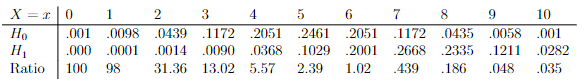
\includegraphics[scale=1.1]{images/hypothesistable.PNG}
\end{figure}

\noindent
Here $H_0$ represents the \textbf{null hypothesis} (that the coin with 0.5 probability is being used), and $H_1$ represents the \textbf{alternative hypothesis} (that the coin with 0.7 probability is being used).
We can specify a \textbf{threshold} $c$ for when we accept or reject the null hypothesis based on the \textbf{ratio} of the probabilities.
For example, if we specify a threshold of $c = 1$ then we \textbf{accept} $H_0$ if $X \leq 6$, and we \textbf{reject} $H_0$ if $X > 6$:

\[ P(\text{reject } H_0 | H_0) = P(X > 6 | H_0) = 0.1675 \text{ } ( \text{sum fields of } H_0 ) \]
\[ P(\text{accept } H_0 | H_1) = P(X \leq 6 | H_1) = 0.3503 \text{ } ( \text{sum fields of } H_1 ) \]

\noindent
\\
For $c = 0.1$ we \textbf{accept} $H_0$ if $X \leq 8$, and we \textbf{reject} $H_0$ if $X > 8$:

\[ P(\text{reject } H_0 | H_0) = P(X > 8 | H_0) = 0.0068 \text{ } ( \text{sum fields of } H_0 ) \]
\[ P(\text{accept } H_0 | H_1) = P(X \leq 8 | H_1) = 0.8506 \text{ } ( \text{sum fields of } H_1 ) \]

\newpage
\noindent
Some terminology:

\begin{itemize}
    \item \textbf{Type I error:} rejecting $H_0$ when it is true
    \item \textbf{Significance Level $\alpha$:} $P(\text{reject } H_0 | H_0)$
    \item \textbf{Type II error:} accepting $H_0$ when it is false
    \item \textbf{$\beta$:} $P(\text{accept } H_0 | H_1)$
    \item \textbf{Power $1 - \beta$:} $P(\text{reject } H_0 | H_1)$
    \item \textbf{Rejection Region:} set of values $X = x$ that lead to rejection of $H_0$
    \item \textbf{Acceptance Region:} set of values $X = x$ that lead to accepting $H_0$
    \item \textbf{Null Distribution:} distribution of $X$ when $H_0$ is true
\end{itemize}

\noindent
\textbf{P-value:} the smallest $\alpha$ for which $H_0$ is rejected.\\
e.g. given $X = 7$, the $p$-value equals $P(X \geq 7 | H_0)$.

\end{document}
